\documentclass[amsthm, twocolumn]{autart}
% Use the option [doublespacing] or [reviewcopy] to obtain double line
% spacing

%%% PACKAGE DECLARATIONS %%%
\usepackage{graphicx}
\usepackage{epstopdf}
\usepackage{amsmath, amssymb, amsfonts, amsopn}
\usepackage{mathrsfs}
\usepackage{psfrag}
%\usepackage[mathscr]{eucal} % Changes \mathcal to use a `fancier' text
\usepackage{euscript}
\usepackage{macros}          % Our own declarations and macros
\usepackage{hyperref}
%\usepackage{dsfont}
\usepackage{dblfloatfix}
%%%%%%%%%%%%%%%%%%%%%%

%%%%% JOURNAL %%%%%%%%
\date{\today}
%%%%%%%%%%%%%%%%%%%%%%


%%%%%%%%%%%%% PDF Stuff
\hypersetup{
pdfauthor = {Alexander Leung},
pdftitle = {ECE 688 Paper: Results and simulations for the global tracking control of underactuated ships by 		Lyapunov's Direct method.},
pdfsubject = {Nonlinear Control Systems},
pdfkeywords = {},
pdfcreator = {\LaTeX with \flqq hyperref \flqq package},
pdfproducer = {dvips + ps2pdf}
}  
%%%%%%%%%%%


%%%%%%%%%%%%%%%%%%%%%%
\begin{document}

%%%%%%%%%%%%%%%%%%%%%%
\begin{frontmatter}
\title{{\sf ECE 688 Paper: Application of Lyapunov's direct method in the design of global tracking controllers for underactuated ships}\thanksref{footnoteinfo}}


\thanks[footnoteinfo]{Corresponding author A. Leung
  Tel. +1.226.868.4286.}


\author[Waterloo]{{\sf Alexander Leung}}

\address[Waterloo]{Department of Electrical and
  Computer Engineering, University of Waterloo, 200 University Ave. W,
  Waterloo, Ontario, N2L 3G1, Canada.}

          
\begin{keyword}                           
nonlinear systems, nonlinear control, ECE 688, project, Lyapunov functions, ship control, global tracking.
\end{keyword}                             
%
%
\begin{abstract}                          % Abstract of not more than 200 words.
This paper studies the results and simulations presented by Jiang (Global tracking control of underactuated ships by Lyapunov's direct method, 2002) in his solution of the global tracking problem for an underactuated ship with only two propellers. Given a condition of persistent excitation, two solutions are proposed by Jiang based on the application of Lyapunuov's direct method. These solutions include (i) a passivity-based design approach; and (ii) a combined cascade-backstepping approach. This paper introduces the global tracking control problem for underactuated ships, presents the major theorems proved by Jiang, and validates the proposed controllers through simulation and comparison.
\end{abstract}
%
%
\end{frontmatter}

%%%%%%%%%%%%%%%%%%%%%%
\section{Introduction}
A control system is called {\sf underactuated} if it has a fewer number of independent actuators than degrees of freedom to be engineered. One such example of an underactuated system is the underactuated ship with two propellers: one being the surge force and the other the yaw moment. This is a rather common form of underactuation that is present in surface vessels involved in off-shore oil field operations.

Prior to the results in Jiang \cite{Jiang02}, the global tracking problem for underactuated ships of the above form was not solved using the existing algorithms of the time. However, many novel nonlinear design techniques existed for the stabilization problem of this underactuated class of ship systems. In Jiang's paper, new solutions to the global asymptotic tracking of underactuated ships were developed by applying Lyapunov's direct method in the controller design.

The purpose of this paper is to present the major results of \cite{Jiang02} and to replicate and expand upon the simulations performed. The design procedure yields controllers which ensure global asymptotic tracking of the underactuated ships and are a result of applying Lyapunov's direct method. These designs also produced explicit Lyapunov functions which are useful in robust and adaptive control design. The first procedure discussed is the use of a passivity-based design technique which is based on the passivity-based $L_gV$ control strategy in \cite{JuQu79}. This yields globally tracking controllers with good transient performance. The second procedure discussed is the use of a combined cascade-backstepping design technique which combines the cascade approach in \cite{Lefe00} with the backstepping design technique in \cite{JiNi99,Jiang00a}. However, this approach yields poorer transient performance when compared to the passivity-based tracking controllers.

The paper is arranged into five sections. Following this introduction, Section 2 describes the necessary background for understanding the underactuated ship problem and outlines the governing system dynamics. Section 3 guides the reader through the major theorems and results derived by Jiang. Section 4 simulates the derived controllers using similar plant conditions as outlined in \cite{Jiang02}. Lastly, Section 5 concludes with a summary of results and main contributions.

%%%%%%%%%%%%%%%%%%%%%%
\section{Background and problem statement}
Consider a surface ship that operates under a failure mode of only two propellers which act on the surge force and yaw torque. Such a configuration which does not include a side force is common due to economic and weight constraints. Under this assumption, the motion of ship dynamics is described by
%
%
\begin{equation}
\begin{aligned}
& \begin{bmatrix} \dot{x} \\  \dot{y} \\  \dot{\psi} \end{bmatrix}
 =
\begin{bmatrix} 
\cos\psi  	& -\sin\psi	 	& 0 \\  
\sin\psi 	& \cos\psi 		& 0\\  
0 		& 0			& 1
\end{bmatrix}
\begin{bmatrix} u \\  v \\  r \end{bmatrix} \\
& \dot{u} =\frac{m_{22}}{m_{11}}vr-\frac{d_{11}}{m_{11}}u+\frac{1}{m_{11}}\tau_s \\
& \dot{v} =-\frac{m_{11}}{m_{22}}ur-\frac{d_{22}}{m_{22}}v \\
& \dot{r} =\frac{m_{11}-m_{22}}{m_{33}}uv-\frac{d_{33}}{m_{33}}r+\frac{1}{m_{33}}\tau_y \\
\end{aligned}
\label{eq:shipsys1}
\end{equation}
%
%
where $(x,y)$ denotes the coordinates of the vessel in the fixed-earth frame, $\psi$ denotes the heading angle of the vessel, and $u$, $v$, and $r$ denote the velocity in surge, sway and yaw respectively. The surge force $\tau_s$ and the yaw torque $\tau_y$ are considered to be the control inputs. The parameters $m_{ii} \ge 0$ and $d_{ii} \ge 0$ are constant and are given by the ship inertia and damping matrices.

The underactuation of this form of ship is seen in the $v$ dynamics of the system (\ref{eq:shipsys1}). In particular, there is no control input (i.e., in the form of a force) to the sway dynamics. This implies that there is no time-invariant state-feedback control law that asymptotically stabilizes the origin. However, time-varying state feedback can meet this challenge. 

In his paper \cite{Jiang02}, Jiang focused on the topic of finding a controller that solves the global tracking problem. That is, given a desired and defined trajectory, find a feedback controller that forces the ship to follow the trajectory from any set of initial conditions. 

The desired trajectory can be generated from the dynamic model of a virtual underactuated ship as follows:
%
%
\begin{equation}
\begin{aligned}
& \begin{bmatrix} \dot{x}_{d} \\  \dot{y}_{d} \\  \dot{\psi}_{d} \end{bmatrix}
 =
\begin{bmatrix} 
\cos\psi_{d}  	& -\sin\psi_{d}	 	& 0 \\  
\sin\psi_{d} 	& \cos\psi_{d} 		& 0\\  
0 			& 0				& 1
\end{bmatrix}
\begin{bmatrix} u_{d} \\  v_{d} \\  r_{d} \end{bmatrix} \\
& \dot{u}_{d} =\frac{m_{22}}{m_{11}}v_{d}r_{d}-\frac{d_{11}}{m_{11}}u_{d}+\frac{1}{m_{11}}\tau_{sd} \\
& \dot{v}_{d} =-\frac{m_{11}}{m_{22}}u_{d}r_{d}-\frac{d_{22}}{m_{22}}v_{d} \\
& \dot{r}_{d} =\frac{m_{11}-m_{22}}{m_{33}}u_{d}v_{d}-\frac{d_{33}}{m_{33}}r_{d}+\frac{1}{m_{33}}\tau_{yd} \\
\end{aligned}
\label{eq:shipsys2}
\end{equation}
%
%
where $(x_{d},y_{d})$ denotes the desired coordinates of the vessel in the fixed-earth frame, $\psi_{d}$ denotes the desired heading angle of the vessel, and $u_{d}$, $v_{d}$, and $r_{d}$ denote the desired velocity in surge, sway and yaw respectively. The reference signals $\tau_{sd}$ and $\tau_{yd}$ are the desired surge force and yaw torque, respectively. Jiang makes an assumption that $(x_{d},y_{d},u_{d},v_{d},r_{d})$ are bounded over $[0,\infty)$, which is a realistic assumption due to the problem physics. Furthermore, a potential energy condition is placed on the desired reference angular velocity:
%
%
\begin{equation}
\begin{split}
& \left(\exists \sigma_{r} > 0\right)(\forall t,t_0\in\Real)(0 \le t_0 \le t < \infty) \\
& \qquad\int_{t_0}^t r_d^2(\tau)\mathrm{d}\tau \geq \sigma_r(t-t_0).
\end{split}
\label{eq:H}
\end{equation}
%
%
This global tracking task described above may be recast into a problem of designing a feedback control law for $(\tau_s,\tau_y)$ so that (\ref{eq:shipsys1}) globally synchronizes with (\ref{eq:shipsys2}). To this end, we simplify systems (\ref{eq:shipsys1}) and (\ref{eq:shipsys2}) by applying the following transform $\Phi$:
%
%
\begin{equation*}
\Phi:(x,y,z)\mapsto\left(z_1,z_2,x_3\right)
\end{equation*}
%
%
where
%
%
\begin{equation*}
\begin{aligned}
& z_1 = x\cos\psi+y\sin\psi \\
& z_2 = -x\sin\psi+y\cos\psi \\
& x_3 = \psi.
\end{aligned}
\end{equation*}
%
%
Applying this transform to both systems (\ref{eq:shipsys1}) and (\ref{eq:shipsys2}) and introducing the error variables,
%
%
\begin{equation*}
\begin{aligned}
& z_{1e}=z_1-z_{1d} \qquad  u_e=u-u_d \\
& z_{2e}=z_1-z_{2d} \qquad  v_e=v-v_d \\
& z_{3e}=z_3-z_{3d} \qquad  r_e=r-r_d \\
\end{aligned}
\end{equation*}
%
%
yields the following system
%
%
\begin{equation}
\begin{aligned}
& \dot{z}_{1e} =u_e+z_{2e}r_d+z_2r_e \\
& \dot{z}_{2e} =v_e+z_{1e}r_d-z_1r_e\\
& \dot{z}_{3e} =r_e \\
& \dot{u}_{e} =\frac{m_{22}}{m_{11}}(vr-v_{d}r_{d})-\frac{d_{11}}{m_{11}}u_{e}+\frac{1}{m_{11}}(\tau_s-\tau_{sd}) \defeq u_1 \\
& \dot{v}_{e} =-\frac{m_{11}}{m_{22}}u_{e}r_{d}-\frac{d_{22}}{m_{22}}v_{e}-\frac{m_{11}}{m_{22}}ur_{e} \\
& \begin{split} \dot{r}_{e} &= \frac{m_{11}-m_{22}}{m_{33}}(uv-u_{d}v_{d})-\frac{d_{33}}{m_{33}}r_{e}+\frac{1}{m_{33}}(\tau_y-\tau_{yd}) \\ & \defeq u_2. \\ \end{split}
\end{aligned}
\label{eq:shipsys3}
\end{equation}
%
%
Observe that the original tracking problem for systems (\ref{eq:shipsys1}) and (\ref{eq:shipsys2}) has been converted to a stabilization problem for system (\ref{eq:shipsys3}). In his paper, Jiang investigates the equivalent problem of global asymptotic stability of the origin for system (\ref{eq:shipsys3}).

%%%%%%%%%%%%%%%%%%%%%%
\section{Control design and major results}

This section discusses the main theorems and results used in designing a controller that ensures the global asymptotic stability of the origin for system (\ref{eq:shipsys3}). 

%% Begin passivity-based control design subsection
\subsection{Passivity-based control design}
\label{sect_passivity}
The first control design strategy that Jiang considers is in exploiting the passivity properties of system (\ref{eq:shipsys3}) and by using the $L_gV$ control strategy previously developed by Jurdjevic \& Quinn in 1979 \cite{JuQu79}. 
%
%
\subsubsection{Design of the surge force $\tau_s$}
\label{sect_passivity_tau_s}
Jiang begins by reducing the problem into two subsystems. The first of which being the $(z_{1e},z_{2e},u_e,v_e)$-subsystem. In this subsystem, $\tau_s$ appears as the input signal to be determined. To design the surge force control law $\tau_s$, consider the following quadratic function:
%
%
\begin{equation}
V_0=\frac{1}{2}(z_{1e} - \lambda_1 z_{2e} r_d)^2 + \frac{1}{2} z_{2e}^2 + \frac{\lambda_0}{2} v_e^2
\end{equation}
%
%
where $\lambda_0$ and $\lambda_1$ are parameters to be designed. The derivative along the $(z_{1e},z_{2e},u_e,v_e)$-subsystem of (\ref{eq:shipsys3}) can be shown to be 
%
%
\begin{equation}
\begin{split}
\dot{V}_0= & (z_{1e} - \lambda_1z_{2e} r_d)[u_e + \lambda_1 r_d^2 (z_{1e} - \lambda_1z_{2e} r_d)  \\
&\!\! - \lambda_1\dot{r}_d z_{2e}  -\lambda_1 r_d (v_e - \lambda_1z_{2e} r_d^2)] - \lambda_1r_d^2 z_{2e}^2 + z_{2e}v_e \\
&\!\! + \lambda_0v_e\bigg(-\frac{m_{11}}{m_{22}}u_e r_d-\frac{d_{22}}{m_{22}} v_e\bigg) + \bigg[ (z_{1e} - \lambda_1 z_{2e} r_d) \\
&\!\! \times (z_2+\lambda_1r_d z_1)-z_{2e} z_1 - \frac{\lambda_0m_{11}}{m_{22}} v_eu \bigg]r_e
\end{split}
\label{eq:V0}
\end{equation}
%
%
To reduce the complexity of the controller equations, a simpler virtual control law $\alpha_0$ is chosen for $u_e$ in (\ref{eq:V0}) as
%
%
\begin{equation}
\alpha_0 = -\lambda_2 (z_{1e} - \lambda_1 z_{2e} r_d)
\end{equation}
%
%
where  $\lambda_2>0$ is a design parameter to be determined later. Define a new variable $\bar{u}_e=u_e-\alpha_0$ and let $\varepsilon \in (0,1)$ be arbitrary.

If the following conditions hold:
%
%
\begin{equation}
\lambda_2 > \lambda_1 \left\lVert r_d \right\rVert^2 \\
\label{eq:suffCond_1}
\end{equation}
\begin{equation}
\begin{split} &(1-\varepsilon)(\lambda_2 - \lambda_1 r_d^2) \\
&\qquad - \bigg( \lambda_0 \lambda_2 \frac{m_{11}}{m_{22}} r_d  - \lambda_1 r_d \bigg)^2 \frac{m_{22}}{2(1-\varepsilon) \lambda_0 d_{22}}  \\
&\qquad \geq \frac{(1-\varepsilon) \lambda_0 d_{22}}{2m_{22}}\lambda_1^2 r_d^3 - \lambda_1 \dot{r_d})^2
\end{split}
\label{eq:suffCond_2}
\end{equation}
%
%
then from (\ref{eq:V0}) it can be shown that 
%
%
\begin{equation}
\begin{split}
\dot{V}_0 \leq \; & \varepsilon(\lambda_2 - \lambda_1 r_d^2)(z_{1e}-\lambda_1 z_{2e} r_d )^2  \\
& - \bigg( \lambda_1 r_d^2 - \frac{m_{22}}{(1-\varepsilon) \lambda_0 d_{22}} \bigg) z_{2e}^2 - \frac{\varepsilon \lambda_0 d_{22}}{m_{22}} v_e^2\\
& + \bigg[ (z_{1e} - \lambda_1 z_{2e} r_d ) - \frac{\lambda_0 m_{11}}{m_{22}} r_d v_e \bigg] \bar{u}_e\\
& + \bigg[ (z_{1e} - \lambda_1 z_{2e} r_d )(z_2 + \lambda_1 r_d z_1 )\\
& - z_{2e} z_1 - \frac{\lambda_0 m_{11}}{m_{22}} v_e u \bigg] r_e.
\end{split}
\end{equation}
%
%
At this point, we introduce the second subsystem. That is, take $u_1$ as the control input and $r_e$ as the disturbance input. Consider the following Lyapunov function candidate for system (\ref{eq:shipsys3}):
%
%
\begin{equation}
\begin{aligned}
V_1 & =  V_0 + \frac{1}{2} \bar{u}_e^2  \\
& = \frac{1}{2}(z_{1e} - \lambda_1 z_{2e} r_d)^2 + \frac{1}{2} z_{2e}^2 + \frac{\lambda_0}{2} v_e^2 \\
&\qquad + \frac{1}{2} (u_e+\lambda_2(z_{1e}-\lambda_1 z_{2e} r_d))^2.
\end{aligned}
\label{eq:V1}
\end{equation}
%
%
If the surge force is selected as
%
%%%% EQUATION 17 FROM JIANG %%%%
\begin{equation}
\begin{split}
\tau_s & = \tau_{sd} + m_{11} \bigg[ -\frac{m_{22}}{m_{11}}(v r-v_d r_d) + \frac{d_{11}}{m_{11}}u_e \\
& -c_1 (u_e + \lambda_2 (z_{1e} - \lambda_1 z_{2e} r_d)) \\ 
& - \bigg ((z_{1e} - \lambda_1 z_{2e} r_d) - \frac{\lambda_0 m_{11}}{m_{22}}r_d v_e \bigg)\\
& - \lambda_2 (u_e + z_{2e} r_d + z_2 r_e) + \lambda_1 \lambda_2 \dot{r}_d z_{2e} + \lambda_1 \lambda_2 r_d \\
& \times (v_e - z_{1e} r_d - z_1 r_e) \bigg] \\
\end{split}
\label{eq:pass_tau_s}
\end{equation}
%
%
with $c_1>0$ as a design parameter, the derivative of $V_1$ along system (\ref{eq:shipsys3}) satisfies:
%
%
\begin{equation}
\begin{split}
\dot{V}_1 \le \; & -c(t) V_1 + \bigg[(z_{1e} - \lambda_1 z_{2e} r_d) (z_2 + \lambda_1 r_d z_1) \\
&\qquad - z_{2e} z_1 - \frac{\lambda_0 m_{11}}{m_{22}} v_e u \bigg] r_e
\end{split}
\label{eq:V1dot}
\end{equation}
%
%
where $c(t)$ is defined by
%
%
\begin{equation}
\begin{split}
c(t) &= \min \bigg\{ 2\varepsilon (\lambda_2-\lambda_1 r_d^2(t)), \\
& \qquad 2\bigg( \lambda_1 r_d^2(t) - \frac{m_{22}}{(1-\varepsilon) \lambda_0 d_{22}}\bigg), 2\varepsilon \frac{d_{22}}{m_{22}}, 2c_1 \bigg\} \\ 
\end{split}
\end{equation}
%
%
Observe that (\ref{eq:V1dot}) implies local exponential stability of the $(z_{1e},z_{2e},u_e,v_e)$-subsystem of (\ref{eq:shipsys3}), which is a motivating result to be used in Section \ref{sect_backstep_yaw}. This completes the passivity-based design procedure for the surge force $\tau_s$.
%
\subsubsection{Design of the yaw moment $\tau_y$}
To design for $\tau_y$, the $L_gV$ design procedure will again be used to create a virtual control law for $r_e$. Once the virtual control law is designed, an application of a integrator backstepping yields the desired $\tau_y$.

Consider the quadratic function
%
%
\begin{equation}
\begin{aligned}
V_2 &= V_1 + \frac{1}{2} z_{3e}^2 \\
&= \frac{1}{2}(z_{1e} - \lambda_1 z_{2e} r_d)^2 + \frac{1}{2} z_{2e}^2 + \frac{\lambda_0}{2}v_e^2 \\
&\qquad + \frac{1}{2} (u_e + \lambda_2 (z_{1e} - \lambda_1 z_{2e} r_d ))^2 + \frac{1}{2} z_{3e}^2.
\end{aligned}
\end{equation}
%
%
The derivative of $V_2$ satisfies
%
%
\begin{equation}
\begin{split}
\dot{V}_2 \le &-c(t) V_1 + \bigg((z_{1e}-\lambda_1 z_{2e} r_d)(z_2 + \lambda_1 r_d z_1) \\
& - z_{2e} z_1 - \frac{\lambda_0 m_{11}}{m_{22}} v_e u + z_{3e}\bigg) r_e\\
\end{split}
\label{eq:V2dot}
\end{equation}
%
%
As in the design of $\tau_s$, choose the following virtual control law $\alpha_1$ for $r_e$ as 
%
%
\begin{equation}
\begin{split}
\alpha_1 = & -c_2 \bigg((z_{1e} - \lambda_1 z_{2e} r_d)(z_2 + \lambda_1 r_d z_1) - z_{2e} z_1 \\
&  - \frac{\lambda_0 m_{11}}{m_{22}} v_e u + z_{3e} \bigg) \\
\end{split}
\end{equation}
%
%
where $c_2>0$ is a design parameter to be determined later. Define a new variable $\bar{r}_e=r_e-\alpha_1$. Then, from (\ref{eq:V2dot}), we have
%
%
\begin{equation}
\begin{split}
\dot{V}_2 \le &-c(t) V_1 -c_2 \bigg((z_{1e} - \lambda_1 z_{2e} r_d)(z_2 + \lambda_1 r_d z_1) \\ 
& -z_{2e} z_1 - \frac{\lambda_0 m_{11}}{m_{22}} v_e u + z_{3e} \bigg)^2 + \bigg((z_{1e} - \lambda_1 z_{2e} r_d) \\
& \times (z_2 + \lambda_1 r_d z_1) - z_{2e} z_1 - \frac{\lambda_0 m_{11}}{m_{22}} v_e u + z_{3e} \bigg) \bar{r}_e
\end{split}
\label{eq:V2dot2}
\end{equation}
%
%
At this point, consider the following Lyapunov function candidate for system (\ref{eq:shipsys3}):
%
%
\begin{equation}
V_3 =  V_2 + \frac{1}{2} \bar{r}_e^2  \\
\label{eq:V3}
\end{equation}
%
%
Observe that $V_3$ is positive definite and radially unbounded in $(t,z_{1e},z_{2e},z_{3e},u_e,v_e,r_e)$. Taking the derivative of $V_3$ along system (\ref{eq:shipsys3}), and using ({\ref{eq:V2dot2}) yields:
%
%
\begin{equation}
\begin{split}
\dot{V}_3 \le & -c(t) V_1 - c_2 \bigg((z_{1e} - \lambda_1 z_{2e} r_d)(z_2 + \lambda_1 r_d z_1) \\
& - z_{2e} z_1 -\frac{\lambda_0 m_{11}}{m_{22}} v_e u + z_{3e} \bigg)^2 + \bar{r}_e \\
& \times \bigg[ \bigg( z_{1e} - \lambda_1 z_{2e} r_d)(z_2 + \lambda_1 r_d z_1) - z_{2e} z_1 \\
& - \frac{\lambda_0 m_{11}}{m_{22}} v_e u + z_{3e} \bigg) + u_2 - \dot{\alpha}_1 \bigg].
\end{split}
\end{equation}
%
%
So, if we select the yaw moment $\tau_y$ to be
%
%%%% EQUATION 26 FROM JIANG %%%%
\begin{equation}
\begin{split}
\tau_y = & \tau_{yd} + m_{33} \bigg[ -\frac{m_{11}-m_{22}}{m_{33}}(uv- u_d v_d) + \frac{d_{33}}{m_{33}} r_e \\
&  -c_3 \bar{r}_e + \dot{\alpha}_1 - ((z_{1e} - \lambda_1 z_{2e} r_d) (z_2 + \lambda_1 r_d z_1)\\
&  -z_{2e} z_1 - \frac{\lambda_0 m_{11}}{m_{22}} v_e u + z_{3e} \bigg) \bigg]\\
\end{split}
\label{eq:pass_tau_y}
\end{equation}
%
%
with $c_3$ a design parameter, it follows that
%
%
\begin{equation}
\begin{split}
\dot{V}_3 \le & -c(t) V_1 - c_2 \bigg((z_{1e} - \lambda_1 z_{2e} r_d)(z_2 + \lambda_1 r_d z_1) \\
& - z_{2e} z_1 -\frac{\lambda_0 m_{11}}{m_{22}} v_e u + z_{3e} \bigg)^2 - c_3 \bar{r}_e^2.
\end{split}
\end{equation}
%
%% Theorem 1 (Global asymptotic tracking)
\subsubsection{Major results}
Motivated by the derivation of controllers in the previous section, Jiang asserts and proves the following Theorem from \cite{Jiang02}.
%
%
\begin{theorem}
(Global asymptotic tracking). Assume that the reference signals $(x_d, y_d, u_d, v_d)$ and $(\tau_{sd},\tau_{yd})$ in (\ref{eq:shipsys2}) are bounded over $[0,\infty)$. Then, if there exist two (sufficiently small) constants $r_\star$ and $r^\star$ such that, for each $t \ge 0$,
%
\begin{equation}
0 < r_\star \le |r_d(t)| \le r^\star \\
\label{eq:thm1cond}
\end{equation}
%
then the problem of global asymptotic tracking is solved for the underactuated ship (\ref{eq:shipsys1}) by the time-varying and Lipschitz continuous state-feedback laws (\ref{eq:pass_tau_s}) and (\ref{eq:pass_tau_y}). In particular, 
%
\[(x_e,y_e,\psi_e,u_e,v_e,r_e)\rightarrow 0 \text{ and }(\tau_s-\tau_{sd},\tau_y-\tau_{yd})\rightarrow 0\]
%
as $t \rightarrow \infty$.
\label{thm1}
\end{theorem}
%
%
Theorem \ref{thm1} is proved in \cite{Jiang02} by Jiang.
%
%
\begin{remark}
By Lyapunov`s first method, the closed-loop system (\ref{eq:shipsys3}), (\ref{eq:pass_tau_s}), and (\ref{eq:pass_tau_y}), is locally exponentially stable at the origin under condition (\ref{eq:thm1cond}).
\end{remark}
%
%
%
%
%% Begin combined cascade-backstepping-based control design subsection
\subsection{Combined cascade-backstepping control design}
The combined-cascade-backstepping control design is a combination of results from the previously derived global asymptotic stabilization of ship tracking systems and a backstepping-based tracking scheme. This produces a new solution to the global tracking problem which leads to global exponential tracking.
%
\subsubsection{Design of the surge force $\tau_s$}
The design of the surge force $\tau_s$ is identical to the derivation performed in Section \ref{sect_passivity_tau_s}. The actual control law is identical to equation (\ref{eq:pass_tau_s}).
%
\subsubsection{Design of the yaw moment $\tau_y$}
\label{sect_backstep_yaw}
In this section, an alternate control law for $\tau_y$ will be derived by using a backstepping technique. The following controller is chosen to stabilize the $(z_{3e},r_3)$-subsystem of (\ref{eq:shipsys3}):
%
%
\begin{equation}
u_2=-k_1 z_{3e} - k_2 r_e
\end{equation}
%
%
where $k_1,k_2>0$ are design parameters. This leads to the following control law for the yaw moment $\tau_y$:
\begin{equation}
\begin{split}
\tau_y=& \tau_{yd}+m_{33} \bigg[-\frac{m_{11}-m_{22}}{m_{33}}(u v - u_d v_d)\\
& + \frac{d_{33}}{m_{33}} r_e - k_1 z_{3e} - k_2 r_e \bigg].
\end{split}
\label{eq:back_tau_y}
\end{equation}
It can be verified that this choice results in global exponential stability at the origin for the $(z_{3e},r_e)$-subsystem of (\ref{eq:shipsys3}). That is, there exist constants $p_1, p_2>0$ such that for any initial condition $(z_{3e}(t_0), r_e(t_0))$ and any initial time $t_0\ge0$, the solution to the $(z_{3e},r_3)$-subsystem of (\ref{eq:shipsys3}) exists and satisfies 
%
%
\begin{equation}
\begin{aligned}
 \left|z_{3e}(t)\right| &\le p_1 e^{-p_2 (t-t_0)} \left|z_{3e}(t_0)\right| \\
 \left|r_e(t)\right| &\le p_1 e^{-p_2 (t-t_0)} \left|r_e(t_0)\right|. \\
\end{aligned}
\label{eq:exp2}
\end{equation}

%
%
%% Theorem 2, 
\subsubsection{Major results}
Motivated by the exponential stability of the individual subsystems (by equations (\ref{eq:V1dot}) and (\ref{eq:exp2})), Jiang asserts and proves the following Theorem from \cite{Jiang02}.
%
%
\begin{theorem}
(Global exponential tracking). Under the assumptions (\ref{eq:H}), (\ref{eq:suffCond_1}), and (\ref{eq:suffCond_2}), the problem of global exponential tracking is solved for the underactuated ship (\ref{eq:shipsys1}) by the time-varying and Lipschitz continuous state-feedback laws (\ref{eq:pass_tau_s}) and (\ref{eq:back_tau_y}). In particular, let 
%
\[X_e \defeq (z_{1e}, z_{2e}, z_{3e}, u_e, v_e, r_e)^\top. \]
%
Then there exist a class-$\kappa$ function $\gamma$ and a constant $\sigma>0$ such that, for any $t_0 \ge 0$ and any $X_e(t_0) \in \Real^6$, the solution $X_e(t)$ exists for each $t \ge t_0$ and satisfies 
%
\begin{equation}
|X_e(t)| \le \gamma(|X_e(t_0)|)e^{-\sigma(t-t_0)}.
\end{equation}

\label{thm2}
\end{theorem}
%
%
Theorem \ref{thm2} is proved in \cite{Jiang02} by Jiang.
%
% Remark 2
\begin{remark}
Since the map $\Phi:(x,y,\psi) \mapsto (z_1,z_2,z_3)$ is a global diffeomorphism with its inverse $\Phi^{-1}$ defined by $\Phi^{-1}=(z_1 \cos z_3- z_2 \sin z_3, z_1 \sin z_3 + z_2 \cos z_3, z_3)$, it can be shown that 
\begin{equation*}
\begin{aligned}
|x(t)-x_d(t)| \rightarrow 0\\
|y(t)-y_d(t)| \rightarrow 0\\
|\psi(t)-\psi_d(t)| \rightarrow 0\\
\end{aligned}
\end{equation*}
at an exponential rate as $t \rightarrow \infty$.
\end{remark}
%
% Remark 3
\begin{remark}
The primary difference between the passivity approach of Section \ref{sect_passivity} and the cascade-backstepping approach of this section is in the way they handle the interconnecting signals between the two LTV systems. A result of this difference is that the passivity approach may result in smaller settling time and an improved transient performance.
\end{remark}
%
% Remark 4
\begin{remark}
In general, Theorem \ref{thm2} does not imply that the closed-loop system (\ref{eq:shipsys3}), (\ref{eq:pass_tau_s}), and (\ref{eq:back_tau_y}) is globally exponentially stable in the sense of Lyapunov since $\gamma$ is not necessarily a linear function. 
\end{remark}
%
%
%% Lemma 1 in Jiang, 2002
%\begin{lemma}
%Consider a first-order differential equation of the form
%%
%%
%\[
%\dot{x}=-(a(t)+f_1(\xi(t)))x+f_2(\xi(t))
%\]
%%
%%
%where $x \in \Real$, $f_1$ and $f_2$ are $C^1$, and $\xi:[0:\infty)\rightarrow \Real^m$ is a time-varying vector-valued signal that exponentially converges to zero and, for all $t \ge t_0 \ge 0$, satisfies
%%
%%
%\[|f_1(\xi(t))| \le \gamma_1(|\xi(t_0)|)e^{-\sigma_1 (t-t_0)}\]
%\[|f_2(\xi(t))| \le \gamma_2(|\xi(t_0)|)e^{-\sigma_2 (t-t_0)}\]
%%
%%
%where $\sigma_1,\sigma_2 > 0$ and $\gamma_1$ and $\gamma_2$ are class-$\kappa$ functions. If there exists a constant $\sigma_3>0$ such that
%%
%%
%\[ (\forall t_2 \ge t_1 \ge 0) \int_{t_1}^{t_2} a(\tau) \mathrm{d}\tau \ge \sigma_3 (t_2-t_1) \]
%%
%%
%then there exists a class-$\kappa$ function $\gamma$ and a constant $\sigma > 0$ such that
%%
%%
%\[ |x(t)| \le \gamma(|x(t_0),\xi(t_0)|)e^{-\sigma (t-t_0)} \]
%%
%%
%\end{lemma}
%
%
%
%%%%%%%%%%%%%%%%%%%%%%
\section{Simulation and performance results}
%
%
% FIGURE 1
\begin{figure*}[!ht]
\begin{center}
\centering 
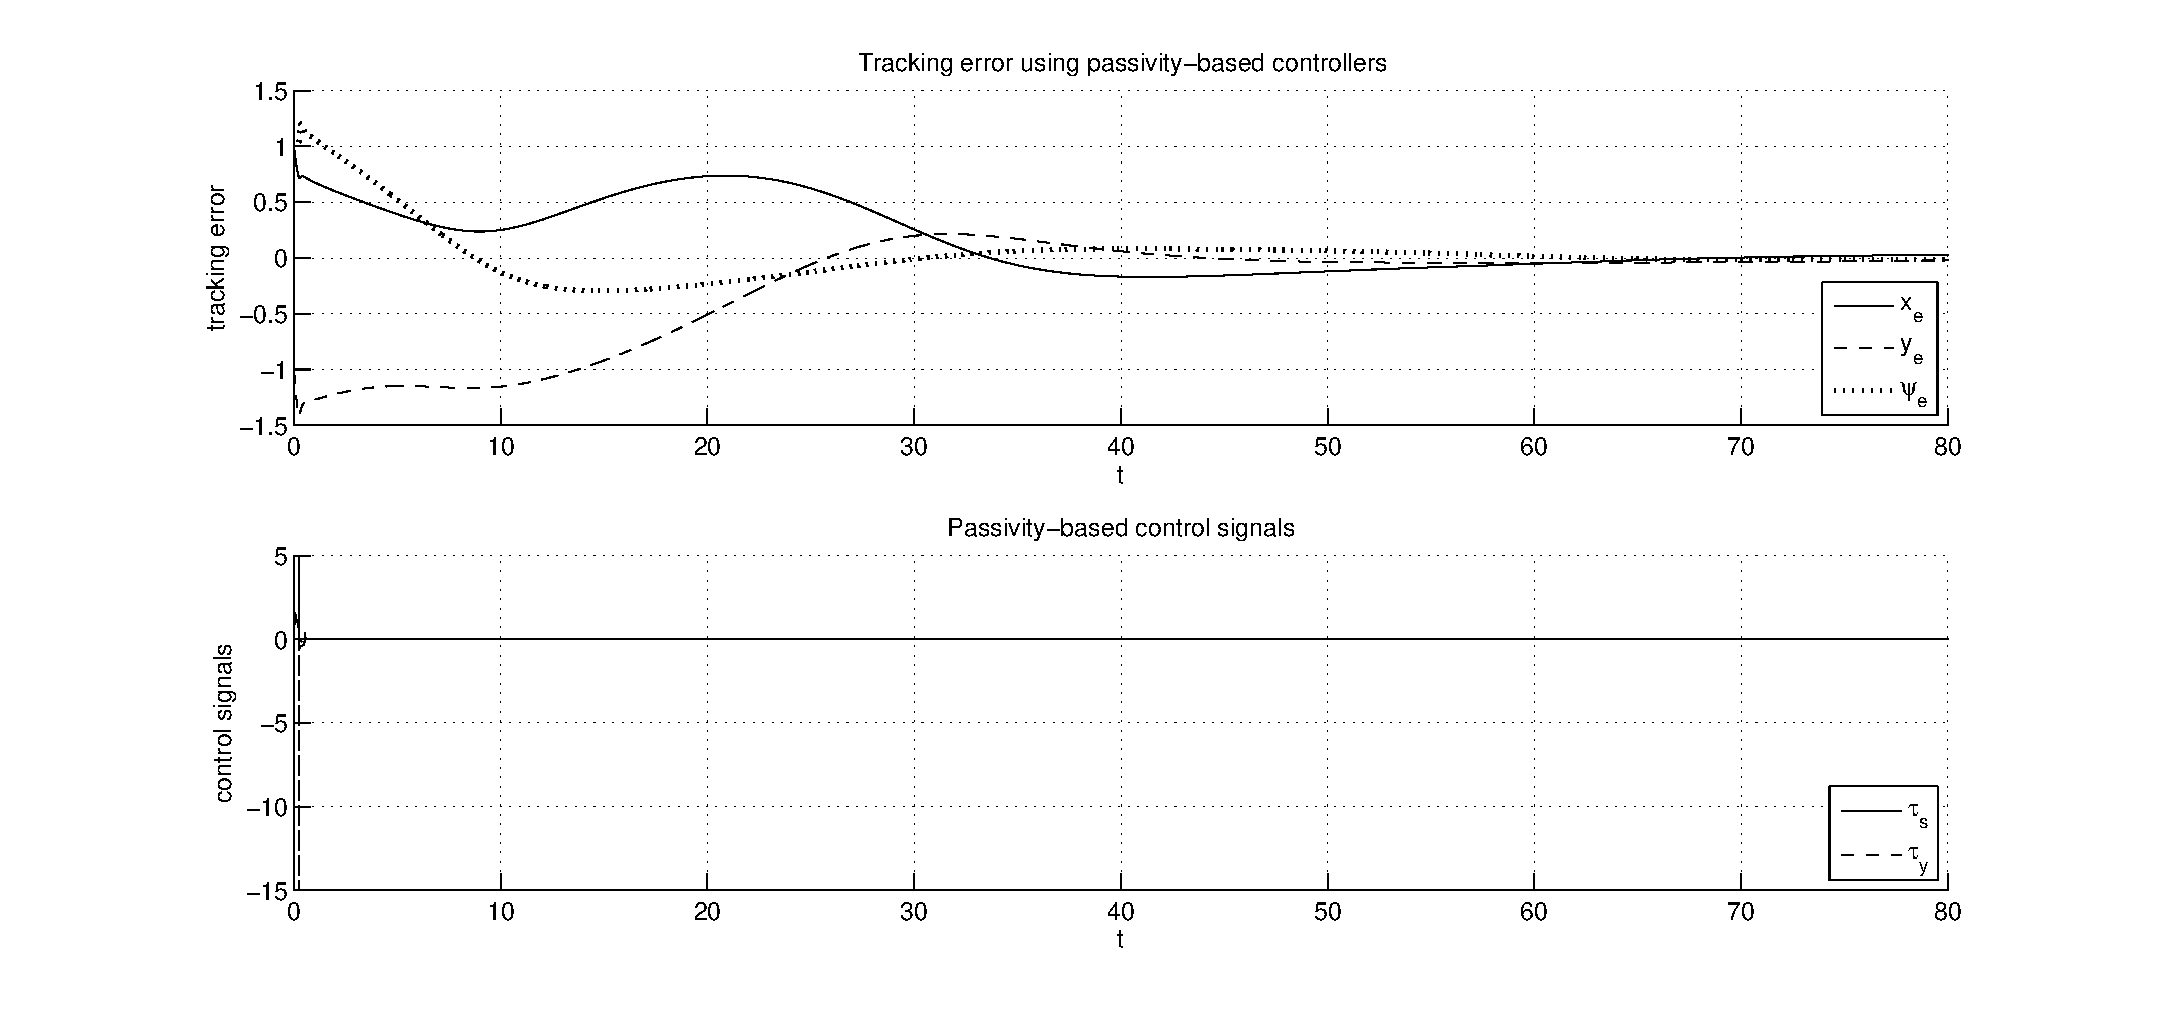
\includegraphics[scale=0.42, trim = 30mm 5mm 30mm 5mm, clip]{FIG_passivity_errors.eps}
\caption{Error signals for the passivity-based tracking controller.}
\label{fig:pass_error}
\end{center}
\end{figure*}
% FIGURE 2
\begin{figure*}[!ht]
\begin{center}
\centering 
\includegraphics[scale=0.42, trim = 30mm 5mm 30mm 5mm, clip]{FIG_backstepping_errors.eps}
\caption{Error signals for the combined-backstepping tracking controller.}
\label{fig:back_error}
\end{center}
\end{figure*}
% %
%
%
This section proceeds by recreating the simulation plots that are shown in \cite{Jiang02} by Jiang. These simulations are performed in MATLAB using the {\sf ODE45} subroutine.

In accordance with the simulation parameters used by Jiang, a circle of radius $1$ was used as the reference trajectory. This was constructed by imposing the following constraints on the reference system:
\begin{equation}
\begin{aligned}
\centering
&(x_d,y_d,\psi_d,u_d,v_d,r_d)|_{t=0}=(0,0,0,0.1,0,0.1) \\
&\dot{u}_d(t)=\dot{v}_d(t)=\dot{r}_d(t)=0 \\
&\tau_{sd}=0.1, \qquad \tau_{yd}=0
\end{aligned}
\end{equation}
Furthermore, as specified in \cite{Jiang02} the simulation uses the following design parameter values: $\lambda_0=10$, $\lambda_1=8$, $\lambda_2=5$, $d_{22}=0.2$, $d_{11}=d_{33}=0$, and $m_{11}=m_{22}=m_{33}=0.1$. 

Note that parameters $c_1$, $c_2$, and $c_3$ in the passivity-based controller were not specified in \cite{Jiang02}. Since the only constraint on these design variables are that they are positive, for the purposes of our simulation we chose $c_1=c_2=c_3=175$ in the control law (\ref{eq:pass_tau_y}). Similarly, the parameters $k_1$ and $k_2$ in the cascade-backstepping-based controller were also not specified in \cite{Jiang02}. This was resolved by choosing $k_1=k_2=50$ in the control law (\ref{eq:back_tau_y}).

The first set of simulations performed were the error signal plots for the ship initial condition of 
%
\[(x,y,\psi,u,v,r)|_{t=0}=(1,-1,1,0,0,0).\]
%
This scenario is identical (up to the choice of design parameters) to the simulation performed by Jiang in \cite{Jiang02}. The passivity-based tracking controller uses equations (\ref{eq:pass_tau_s}) and (\ref{eq:pass_tau_y}) while the cascade-backstepping tracking controller uses equations (\ref{eq:pass_tau_s}) and (\ref{eq:back_tau_y}). The error plots over time for the passivity-based and cascade-backstepping-based controllers are shown in Figure \ref{fig:pass_error} and Figure \ref{fig:back_error}, respectively. Observe that the passivity-based controller yields better transient performance while the cascade-backstepping-based controller has better asymptotic properties. Furthermore, these plots have the same shape and form of those shown in \cite{Jiang02}, as expected.

In addition to the error plots, the phase plots for each control scheme at varying initial ship conditions further illustrate the transient and asymptotic properties. These are shown in \ref{fig:pass_traj} and Figure \ref{fig:back_traj}. These plots were not provided by Jiang in his original paper.
%
% FIGURE 3
\begin{figure*}[!h!t]
\begin{center}
\centering 
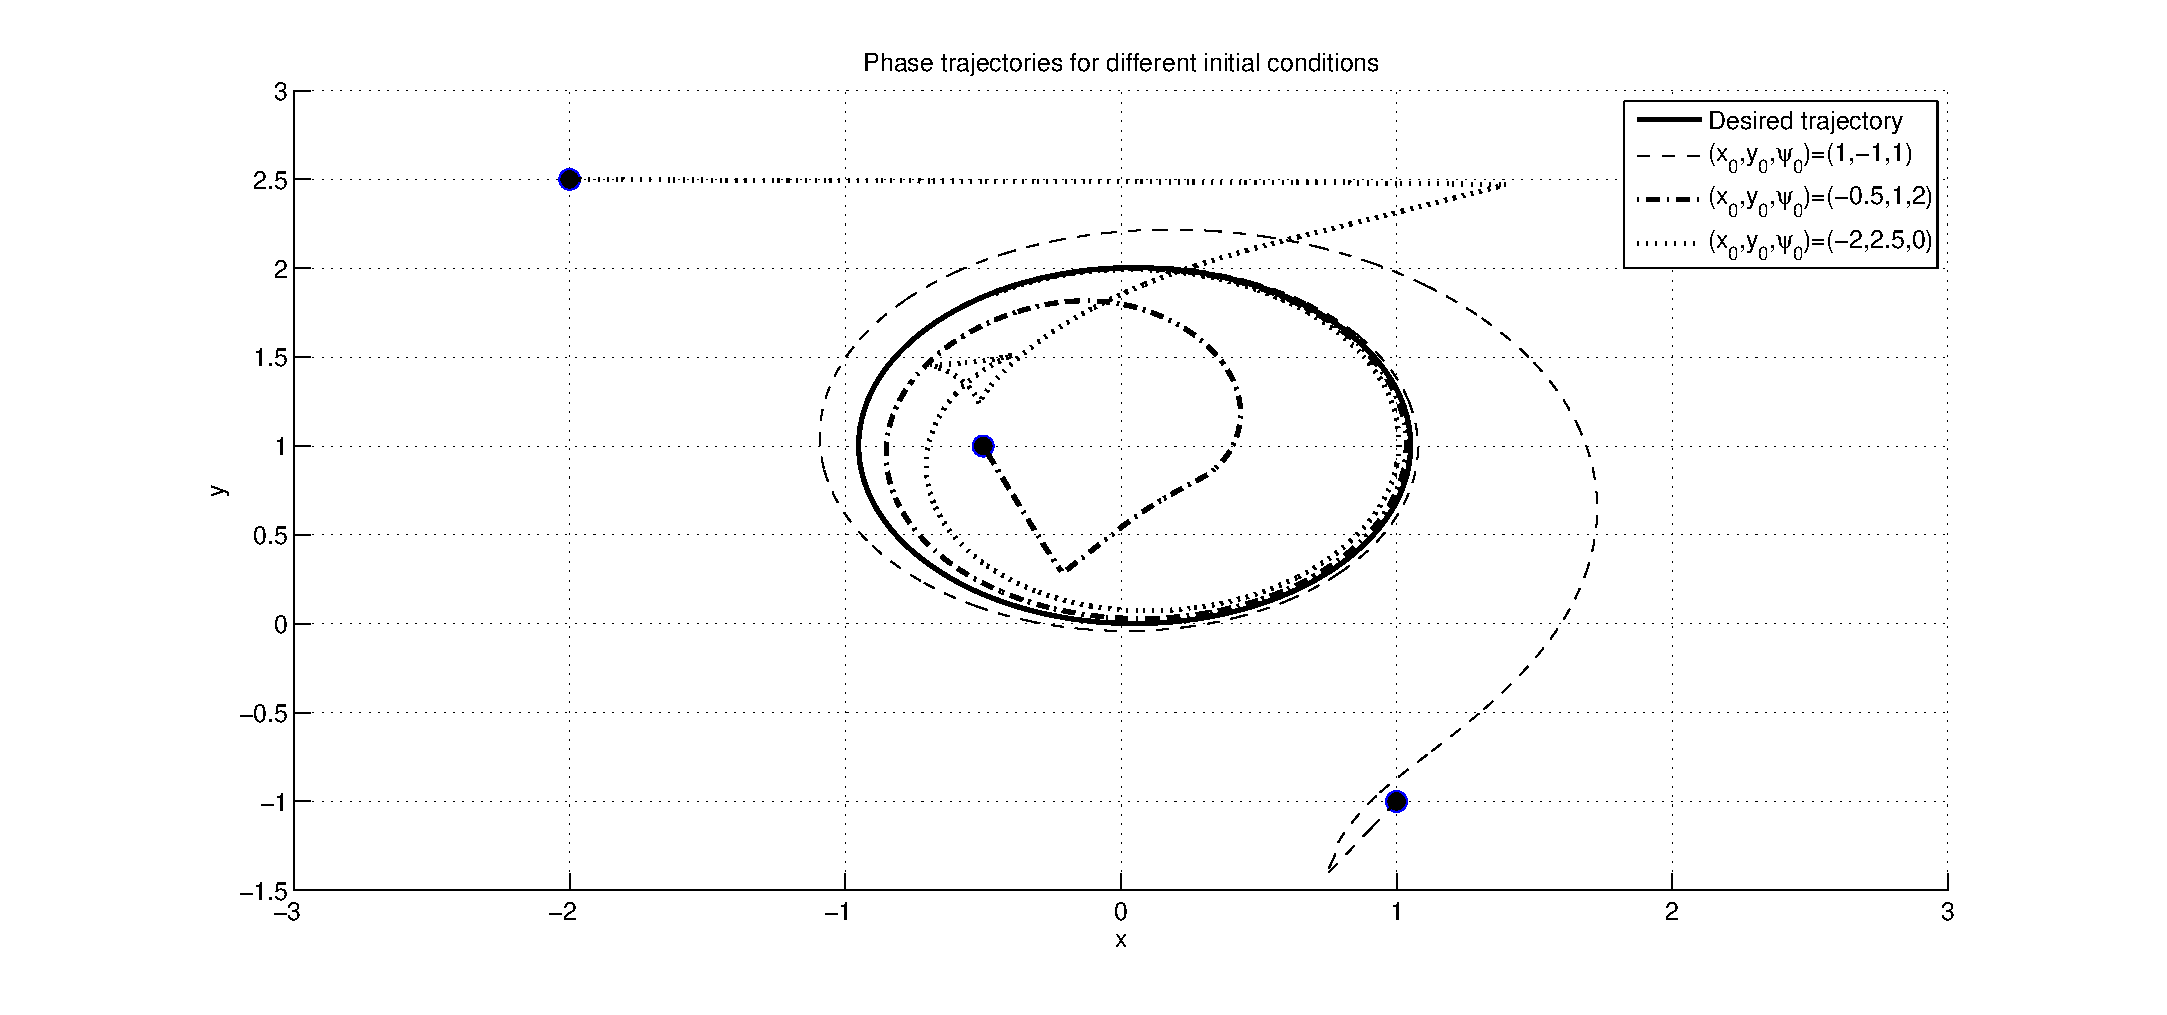
\includegraphics[scale=0.41, trim = 30mm 5mm 30mm 5mm, clip]{FIG_passivity_trajectories.eps}
\caption{Phase plots for the passivity-based tracking controller with varying initial conditions.}
\label{fig:pass_traj}
\end{center}
\end{figure*}
% FIGURE 4
\begin{figure*}[!h!t]
\begin{center}
\centering 
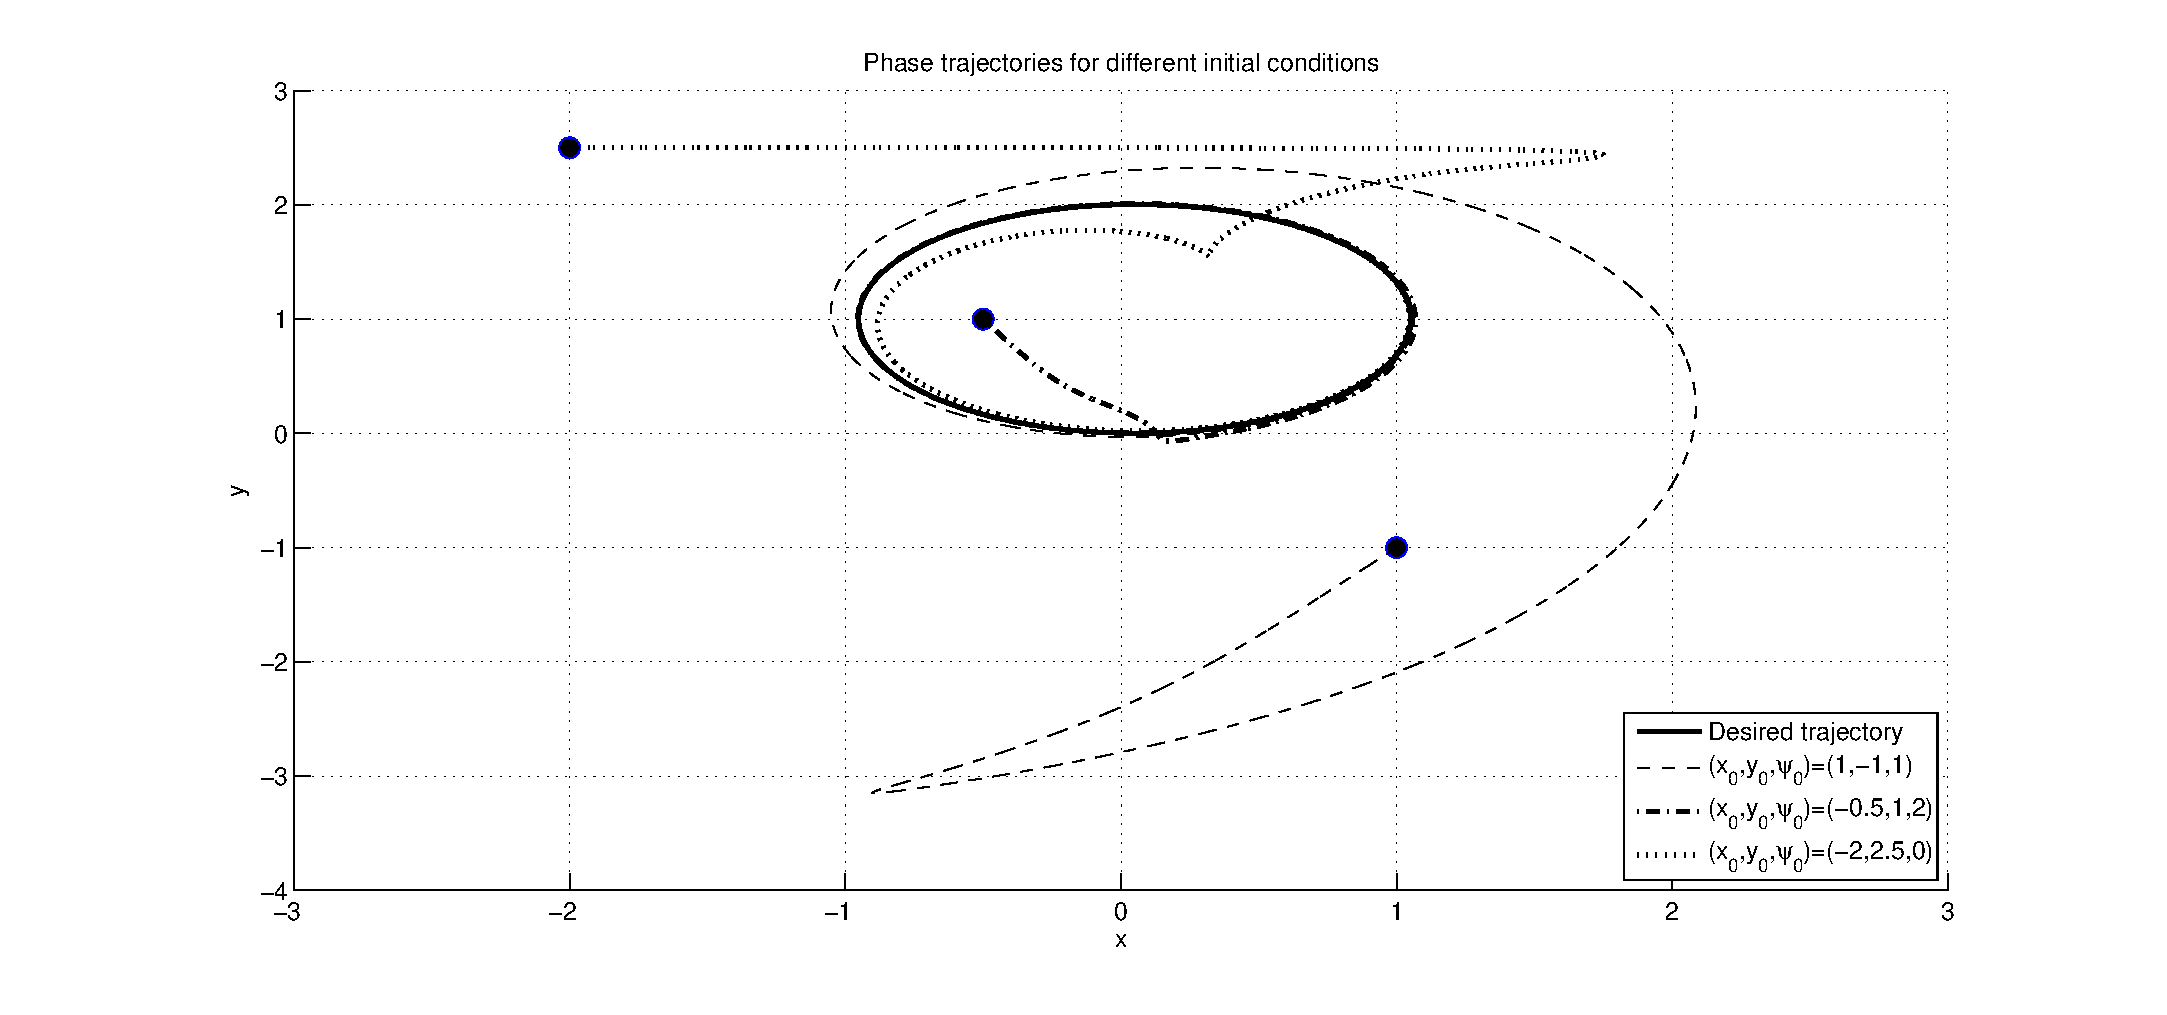
\includegraphics[scale=0.41, trim = 30mm 5mm 30mm 5mm, clip]{FIG_backstepping_trajectories.eps}
\caption{Phase plots for the combined-backstepping tracking controller with varying initial conditions.}
\label{fig:back_traj}
\end{center}
\end{figure*}
%
%
%
%%%%%%%%%%%%%%%%%%%%%%
\section{Conclusions, critique, and future work}
%
This paper has summarized and restated the key results and findings from Jiang in his paper \cite{Jiang02}. Furthermore, the author of this paper has simulated the control laws derived by Jiang and has observed similar responses in terms of transient and asymptotic behaviour. In addition, the results from Theorem \ref{thm1} and Theorem \ref{thm2} were verified and the global convergence of each controller shown by simulating the system at various initial conditions. In particular, we see global asymptotic tracking from (\ref{eq:pass_tau_s}) and (\ref{eq:pass_tau_y}) while we see global exponential tracking from (\ref{eq:pass_tau_s}) and (\ref{eq:back_tau_y}).

Although Jiang is correct in stating that the controllers have global asymptotic tracking, the transient performance of these controllers do not have adequate performance. From the original plots described in \cite{Jiang02} (i.e., the plots of the error signals) it shows that the tracking is smooth, but does not reveal information about the actual path that is simulated. From Figure \ref{fig:pass_traj} and Figure \ref{fig:back_traj}, it is clear that there are unrealistic ship trajectories for some initial conditions. This is due to the simplified model used in the simulation (with $d_{11}=d_{33}=0$) which was implemented to match the conditions described in Jiang's paper. 

A topic of future study is to examine the behaviour of the transient and asymptotic behaviour as the model parameters are varied. That is, studying the performance of each controller as parameters $d_{11}$, $d_{22}$, $d_{33}$, $m_{11}$, $m_{22}$, and $m_{33}$ change.
%
%%%%%%%%%%%%%%%%%%%%%%.
%%%%%%%%%%%%%%%%%%%%%%
%%%%%%%%%%%%%%%%%%%%%%
%%%%%%%%%%%%%%%%%%%%%%
%
%
%\begin{equation}
%\begin{aligned}
%\dot{x} = f(x) + g(x)u,
%\end{aligned}
%\label{eq:system}
%\end{equation}
%%
%%
%where $x \in \Real^n$ is the state and $u \in \Real$ is the control
%input. The vector fields $f, g: \Real^n \rightarrow T\Real^n$ are
%smooth ($C^\infty$). 
%
%\begin{definition}
%The {\sf tangent bundle} $TM$ of a manifold $M$ given by
%%
%%
%\[
%TM \eqdef \bigcup_{p \in M}T_pM \qquad (\text{disjoint union}).
%\]
%%
%%
%An element of $TM$ can be taken to be a pair $(p, \left[c\right]_p)$,
%with $p \in M$ and $\left[c\right]_p \in T_pM$. The map $\pi : TM
%\rightarrow M$, $(p, \left[c\right]_p) \mapsto p$, is called the {\sf
%natural projection} of $TM$ onto $M$.
%\end{definition}
%
%The tangent bundle is a manifold in its own right. It has a natural
%manifold structure induced by the differentiable structure of $M$. It
%has dimension $2m$.
%
%\begin{definition}
%Let $p$ be a point of a manifold $M$. The {\sf cotangent space}
%$T^\star_pM$ is the dual space of $T_pM$, i.e., the set of all linear
%functionals
%%
%%
%\[
%\begin{aligned}
%\sigma(p): &T_pM\rightarrow \Real.
%\end{aligned}
%\]
%%
%%
%Elements of the cotangent space are called {\sf tangent
%  covectors}. The {\sf cotangent bundle} of $M$ is defined as
%%
%%
%\[
%T^\star M \eqdef \bigcup_{p \in M}T^\star_pM \qquad (\text{disjoint
%union}).
%\]
%%
%%
%\label{def:cotangentspace}
%\end{definition}
%
%The cotangent bundle can be given a manifold structure using the
%differentiable structure on $M$, in much the same way as the tangent
%bundle. Next we define the notion of a vector field and covector
%field.
%
%\subsection{Local representations}
%
%Let $(W, \psi)$ be an admissible coordinate chart on the manifold
%$M$. Recall that the differentiable structure on $M$ induces a natural
%basis of the tangent space $T_pM$ at each $p \in W$ as follows.
%
%\section{Derived systems}
%\label{sec:mysection}
%
%Let $\Sigma$ be a given Pfaffian system of constant
%rank~\cite{Jiang02,BryCheGarGolGri90,GarSha90}.
%
%
%
%%%%%%%%%%%%%%%%%%%%%%
%%%%%% BIBLIOGRAPHY %%%%%%%%%%%
\bibliographystyle{elsart-num}
%\bibliographystyle{plain}
\bibliography{yourbib}
%%%%%%%%%%%%%%%%%%%%%%%%%%%%%%%
\end{document}
